%=====================================================================
\chapter{Research Methodology and Proposed System Implementation}
%=====================================================================

This chapter develops the methodology objective by objective. For each objective it states
the design, describes the implementation as an ordered engineering procedure, presents the
experimental evidence, and records the publication in which the work was validated.
Section~5.6 then shows how the four components compose into a single system.

\section{Overall Research Framework and Workflow}

The framework is organised as the four layers of Figure~\ref{fig:context}. Each layer consumes
the output of the previous one and each corresponds to one research objective, so that a defect
in any layer can be located rather than absorbed into an aggregate performance figure. Layer~0
acquires four heterogeneous streams and aligns them to a common trading calendar without
look-ahead. Layer~1 (RO1) encodes each modality and fuses them under cross-modal attention and
then under measured source reliability. Layer~2 (RO2) applies the optimised deep architecture
that turns the fused representation into a prediction. Layer~3 (RO3) supplies the transparency
instruments --- directed causal structure and sentiment diagnostics --- and returns a
reliability revision to the fusion layer, so that a source found to be noisy is down-weighted
rather than merely reported. Layer~4 (RO4) converts the signal into an allocation under risk,
cost and turnover constraints and validates it by walk-forward testing, a specification sweep,
matched-exposure ablation, a holdout and a second market. The sequence was executed once end to
end and then revisited iteratively as each objective produced evidence that constrained the
next.

Two deliberate design decisions govern the data. The study universes differ by objective
because the objectives ask different questions: sectoral breadth is required to test fusion
(NIFTY~50 and ten sectoral indices, January 2015 to December 2024, with fifteen technical
indicators, financial press, X and StockTwits, and RBI, MOSPI and IMF macroeconomic series);
single-name depth is required to test sentiment (Indian large-capitalisation equities with
daily OHLCV and news headlines scored by a transformer); a compact cross-sectional universe is
required to recover causal structure (five NIFTY50 constituents across five sectors, 308
sessions from January 2024); and cross-asset volatility dispersion is required to test
allocation (ten multi-asset instruments over 4,689 sessions from January 2008, with a secondary
mega-capitalisation universe). And the evaluation window lengthens as the objectives progress,
from a ten-year sectoral study to an eighteen-year multi-asset study with a dedicated holdout,
because claims about behaviour under market stress require observations of market stress. Each
study uses the protocol appropriate to its question --- chronological splitting with
training-set-only standardisation and expanding-window walk-forward for RO1 and RO2,
conditional independence testing for RO3, and 21-session walk-forward with 10\,bp transaction
costs, an 18-cell specification sweep, matched-exposure ablation and a 665-session holdout for
RO4.

%---------------------------------------------------------------------
\section{Proposed Methodology for Research Objective 1}

\textbf{RO1:} \emph{To investigate and develop a comprehensive model that integrates diverse
data sources --- financial metrics, news articles, social media sentiment and macroeconomic
factors --- aiming to enhance the accuracy of stock market predictions.}

\subsection{Design and implementation of the multi-source fusion network}

The Multi-Source Fusion Network is a hierarchical architecture that learns modality-specific
representations before learning cross-modal ones, so that each stream is encoded in a form
appropriate to its own structure (Figure~\ref{fig:msfn}). \textbf{(1)~Acquire and align:}
collect price and volume records, news articles, social media posts and macroeconomic releases
and align every stream to the trading calendar; monthly and quarterly macroeconomic series are
interpolated to daily frequency, and the consequence --- an understatement of discontinuous
announcement-day effects --- is stated explicitly rather than left implicit.
\textbf{(2)~Engineer modality features:} derive fifteen technical indicators covering trend,
momentum, volatility and volume; score news articles with a domain-adapted transformer encoder
weighted by relevance and source authority; score social media posts with a hybrid lexicon and
fine-tuned recurrent classifier, retaining daily polarity, mention volume and dispersion;
normalise the macroeconomic series. \textbf{(3)~Encode each modality} by one-dimensional
convolution, with $h_m^{(l)}$ the representation of modality $m$ at layer $l$:
$h_m^{(l)} = \mathrm{ReLU}(\mathrm{Conv1D}(W_m^{(l)} * h_m^{(l-1)} + b_m^{(l)}))$.
\textbf{(4)~Fuse by cross-modal attention:} compute a relevance weight
$\alpha_m = \mathrm{softmax}(q \cdot k_m / \sqrt{d_k})$ per modality, where $q$ is a learned
query vector, $k_m$ the key vector of modality $m$ and $d_k$ the key dimension; the weights are
recomputed at each time step, which is what allows source importance to move with the market
state. \textbf{(5)~Model temporal dependence:} pass the fused representation $F_t$ through
bidirectional recurrent layers, $h_t = [\overrightarrow{h}_t ; \overleftarrow{h}_t]$ with
$\overrightarrow{h}_t = \mathrm{LSTM}(F_t, \overrightarrow{h}_{t-1})$ and
$\overleftarrow{h}_t = \mathrm{LSTM}(F_t, \overleftarrow{h}_{t+1})$, and produce forecasts at
horizons $\tau \in \{1,3,7,15\}$ days through dense layers with
dropout~\cite{srivastava2014dropout}, trained by adaptive moment
estimation~\cite{kingma2015adam} with early stopping. \textbf{(6)~Evaluate without leakage:}
partition chronologically into training (2015--2021), validation (2022 -- mid-2023) and test
(mid-2023 -- 2024) blocks, standardise using training-set statistics only, tune hyperparameters
on the validation block alone, and fix random seeds so that reported differences reflect
architecture rather than initialisation.

\begin{figure}[!htb]
\centering
\scalebox{0.72}{\begin{tikzpicture}[node distance=3mm]
\node[blkd,minimum width=25mm,minimum height=8mm] (d1) {Financial data\\NSE / BSE};
\node[blkd,right=3mm of d1,minimum width=25mm,minimum height=8mm] (d2) {News articles\\financial press};
\node[blkd,right=3mm of d2,minimum width=25mm,minimum height=8mm] (d3) {Social media\\X, StockTwits};
\node[blkd,right=3mm of d3,minimum width=25mm,minimum height=8mm] (d4) {Macro data\\RBI, MOSPI};

\node[blk,below=6mm of d1,minimum width=25mm,minimum height=8mm] (p1) {15 technical\\indicators};
\node[blk,below=6mm of d2,minimum width=25mm,minimum height=8mm] (p2) {Transformer\\sentiment scoring};
\node[blk,below=6mm of d3,minimum width=25mm,minimum height=8mm] (p3) {Lexicon + LSTM\\sentiment scoring};
\node[blk,below=6mm of d4,minimum width=25mm,minimum height=8mm] (p4) {Normalisation and\\daily interpolation};

\node[blkg,below=6mm of p1,minimum width=25mm,minimum height=8mm] (e1) {CNN\\feature maps};
\node[blkg,below=6mm of p2,minimum width=25mm,minimum height=8mm] (e2) {Text\\embeddings};
\node[blkg,below=6mm of p3,minimum width=25mm,minimum height=8mm] (e3) {Text\\embeddings};
\node[blkg,below=6mm of p4,minimum width=25mm,minimum height=8mm] (e4) {Temporal\\features};

\node[blka,below=7mm of e2,minimum width=79mm,minimum height=8mm,xshift=14mm] (att)
  {Cross-modal attention $\;\to\;$ concatenation $\;\to\;$ adaptive weighting};
\node[blka,below=5mm of att,minimum width=79mm,minimum height=8mm] (bl)
  {Bi-LSTM encoder with temporal attention $\;\to\;$ dense layers with dropout};
\node[blkd,below=5mm of bl,minimum width=79mm,minimum height=7mm] (o)
  {Predicted level and direction with confidence interval, horizon $\tau \in \{1,3,7,15\}$ days};

\foreach \a/\b in {d1/p1,d2/p2,d3/p3,d4/p4,p1/e1,p2/e2,p3/e3,p4/e4}
  \draw[ar] (\a) -- (\b);
\foreach \a in {e1,e2,e3,e4} \draw[ar] (\a.south) -- ++(0,-2mm) -| (att.north);
\draw[ar] (att) -- (bl);
\draw[ar] (bl) -- (o);
\node[lbl,rotate=90,anchor=center,align=center]
  at ([xshift=-7mm]$(d1.west)!0.5!(e1.west)$)
  {acquisition, preprocessing\\and feature extraction};
\node[lbl,rotate=90,anchor=center] at ([xshift=-7mm]d1.west |- att) {fusion};
\node[lbl,rotate=90,anchor=center] at ([xshift=-7mm]d1.west |- o) {output};
\end{tikzpicture}}
\caption[Architecture of the Multi-Source Fusion Network]{Architecture of the Multi-Source
Fusion Network, showing the flow from heterogeneous acquisition through modality-specific
preprocessing and feature extraction to cross-modal fusion and prediction.}
\label{fig:msfn}
\end{figure}

\subsection{Results and discussion for Research Objective 1}

Table~\ref{tab:msfn} reports the comparison against six baselines together with the source
ablation, presented as one table because the two questions --- does fusion help, and which
source is responsible --- are answered by the same experiment.

\begin{table}[!htb]
\centering
\caption[Prediction performance and source ablation on the NIFTY 50 index]{One-day-ahead
prediction on the NIFTY 50 index: comparison against baselines (upper block) and source
ablation of the proposed model (lower block)}
\label{tab:msfn}
\tabfont
\begin{tabular}{@{}L{4.6cm}L{3.3cm}rrrr@{}}
\toprule
\textbf{Configuration} & \textbf{Data sources} & \textbf{MAE} & \textbf{RMSE} &
\textbf{$R^2$} & \textbf{DA (\%)} \\
\midrule
\multicolumn{6}{@{}l@{}}{\textit{Baseline comparison}}\\
ARIMA & price only & 0.124 & 0.167 & 0.721 & 52.3 \\
LSTM & price only & 0.087 & 0.112 & 0.845 & 61.7 \\
Transformer & price only & 0.079 & 0.103 & 0.869 & 64.2 \\
LSTM + sentiment & price, sentiment & 0.052 & 0.071 & 0.921 & 72.8 \\
LSTM + macro & price, macro & 0.061 & 0.082 & 0.903 & 68.5 \\
Ensemble (simple average) & all, fixed weights & 0.043 & 0.059 & 0.942 & 76.3 \\
\textbf{MSFN (proposed)} & \textbf{all, adaptive fusion} & \textbf{0.018} &
\textbf{0.024} & \textbf{0.988} & \textbf{84.7} \\
\midrule
\multicolumn{6}{@{}l@{}}{\textit{Source ablation of the proposed model}}\\
$-$ financial metrics & news, social, macro & 0.041 & 0.055 & 0.946 & 73.2 \\
$-$ news sentiment & price, social, macro & 0.027 & 0.036 & 0.971 & 79.1 \\
$-$ social media & price, news, macro & 0.025 & 0.033 & 0.976 & 80.8 \\
$-$ macroeconomic & price, news, social & 0.031 & 0.040 & 0.965 & 76.5 \\
$-$ both sentiment sources & price, macro & 0.038 & 0.049 & 0.952 & 74.0 \\
price and technical only & price only & 0.079 & 0.103 & 0.869 & 64.2 \\
\bottomrule
\end{tabular}
\end{table}

Three readings follow. First, adaptive fusion is materially better than fixed-weight
combination: the simple averaging ensemble uses exactly the same four sources and attains a
mean absolute error of 0.043 against 0.018, which isolates the contribution of the weighting
rule rather than of the data. Second, financial metrics remain foundational --- their removal
costs 22.6 per cent of explained variance --- but they are not sufficient, since restricting the
model to price and technical features costs 32.0 percentage points of directional accuracy.
Third, the joint removal of both textual sources costs 10.9 per cent of explained variance,
exceeding the sum of their individual removals of 5.3 and 3.6 per cent; that superadditivity is
the quantitative signature of complementary rather than redundant information, and it is the
empirical justification for a fusion architecture instead of a larger single-source model.

The learned attention distribution explains where the gain comes from. Financial metrics carry
the highest average weight at 35 per cent, rising to 42 per cent during earnings season, when
company-specific numerical disclosure dominates, and falling to 28 per cent under high
volatility, when the social media weight rises from 18 to 28 per cent; news sentiment averages
22 per cent and macroeconomic indicators 25 per cent, so the textual sources jointly carry 40
per cent. This is precisely the behaviour a fixed-weight scheme cannot reproduce, and it is
consistent with the finding that social media sentiment influences Indian sectoral returns most
strongly at market extremes~\cite{khan2025asymmetric}. Because the headline accuracy is high,
the possibility that it is an artefact of a fortunate split was tested under an expanding-window
protocol in which each fold is evaluated only on sessions strictly later than its training
window. Normalised errors are tightly clustered at $0.0016 \pm 0.0004$ and directional accuracy
remains above chance in every fold, ranging from 68 to 92 per cent with a mean of 78.4 per cent;
fold-level $R^2$ averages 0.874, naturally lower than the full-test value because each short
window spans a narrow price range, and the stability of the error magnitudes, not the level of
$R^2$, is the relevant evidence. Sector-wise evaluation adds a second dimension: financials and
fast-moving consumer goods are the most predictable at $R^2$ above 0.985 while metals and real
estate fall below 0.962, and sentiment contributes most to the globally exposed information
technology and pharmaceutical sectors whereas energy and metals depend more heavily on
macroeconomic indicators. Source importance is therefore structured by sector as well as by
regime.

\subsection{Strengthening the fusion rule: dynamic uncertainty weighting}

Attention weights are learned once over a training set and express \emph{average relevance}
rather than \emph{instantaneous reliability}: a source that has become unreliable in the last
two weeks continues to receive its historical weight. To remove that limitation the fusion rule
was reformulated on a Bayesian basis. Each source $i \in \{M, S, A\}$ --- market series,
sentiment sequence, volatility index --- is modelled by an expert network matched to its
structure: a gated recurrent unit, a transformer encoder and a multi-layer perceptron
respectively. The predictive uncertainty $\sigma_{i,t}^2$ is estimated as the variance of that
expert's prediction errors over a trailing window of $\tau = 10$ sessions, and the
uncertainties are converted into fusion weights by a softmax over their negatives, so that the
fused forecast $\hat{y}_t = \sum_i w_{i,t}\hat{y}_{i,t}$ uses
\begin{equation}
w_{i,t} = \frac{\exp\!\left(-\sigma_{i,t}^2 / T\right)}
               {\sum_j \exp\!\left(-\sigma_{j,t}^2 / T\right)},
\end{equation}
with $T$ a temperature parameter: a source whose recent error variance has risen is
automatically down-weighted. Distribution-aware normalisation is applied throughout ---
standard scaling for returns, min--max for sentiment, robust scaling for the heavy-tailed
volatility index --- fitted on an expanding window so that no future information enters the
scaler.

The mechanism self-corrects in a way a static scheme cannot: if a sentiment score is distorted
by an ambiguous or ironic headline and the subsequent market move contradicts it, the error
enters $\sigma_{S,t}^2$ and the sentiment weight falls over the following sessions without
manual intervention. This is the direct methodological answer to gap G1. The formulation was
evaluated on a heterogeneous Nifty~50 dataset spanning January 2018 to December 2023: index
price and volume records with fifteen technical indicators, a daily sentiment score from a
language model fine-tuned on Indian financial news, and the India VIX as an alternative source
of forward-looking volatility. News sentiment is assigned to the next National Stock Exchange
session so that lagged market impact is captured without look-ahead, market holidays are treated
as genuine gaps rather than forward-filled, and the split is strictly sequential ---
2018--2021 training, 2022 validation, 2023 out-of-sample test --- with the experts pre-trained
independently and the system then fine-tuned end to end through the fusion layer.
The comparison is against the three static fusion strategies identified in Chapter~2: early
fusion, in which all sources are concatenated into one recurrent model and the weights are
fixed by the architecture~\cite{moodi2024}; late fusion, in which the three expert predictions
are averaged with pre-determined weights~\cite{farimani2024}; and attention fusion, in which
static neural attention over modalities is learned once and then held
fixed~\cite{liu2019attention,haryono2023} --- the strongest of the three. A fourth
configuration, the proposed architecture with the uncertainty term disabled, isolates the
weighting rule from the expert networks. The source study reports improvements relative to the
strongest baseline rather than absolute levels.

Two readings follow. Against the strongest static competitor the dynamic rule improves the
Sharpe ratio by 22.7 per cent and reduces maximum drawdown by 18.3 per cent, so the gain is in
risk-adjusted terms and downside control rather than in raw accuracy. The second reading matters
more: the ablation row shows that the same three expert networks, fused with fixed weights,
perform no better than the established baselines. The experts are therefore not the source of
the improvement; the weighting rule is --- which allows the contribution to be stated precisely
as a fusion-mechanism result rather than an architecture result, and is the same style of
component-level attribution that Objective~4 later applies to the allocation layer. The
behaviour is interpretable in the way the design intends: during the volatility episodes in the
test window the weight on the technical expert falls as its recent error variance rises and
migrates to the volatility-index expert and, less strongly, to the sentiment expert, returning
in calmer trending stretches. Because the shift is driven by measured error variance rather than
by a learned prior, no regime label is required for it to occur.

\subsection{Summary and validation of Research Objective 1}

The objective is achieved. A four-stream model evaluated on ten years of Indian market data
across ten sectors attains MAE 0.018, $R^2$ 0.988 and directional accuracy 84.7 per cent
against 76.3 per cent for a fixed-weight ensemble over identical inputs; ablation demonstrates
that textual sources contribute superadditively and the attention analysis that source
importance is regime-dependent. The fusion rule was then strengthened from learned average
relevance to measured instantaneous reliability, closing the static-weighting gap.
\pubcite{P1} supplies the architecture, the ten-sector evaluation, the ablation and the
walk-forward analysis; \pubcite{P4} supplies the uncertainty formulation and the dynamic
weighting mechanism.

%---------------------------------------------------------------------
\section{Proposed Methodology for Research Objective 2}

\textbf{RO2:} \emph{To design a hybrid framework that combines large language models,
sentiment analysis techniques and conventional financial indicators, focusing on optimising
deep learning architectures for real-time stock market predictions.}

\subsection{Design and implementation of the hybrid LLM--indicator framework}

The framework is organised as five interconnected layers --- data collection, technical
indicators, sentiment analysis, feature fusion, and model training with evaluation. Its design
priority differs from that of Objective~1: rather than maximising the number of sources, it
isolates one source --- news text read by a transformer language model --- and measures
precisely what that source adds to a conventional indicator set. Daily price and volume records
are retrieved for the target equities and financial news headlines are harvested with
non-financial content filtered out and credible sources prioritised; publication timestamps are
synchronised with session times so that news released after the close is attributed to the next
trading day. Fifteen indicators are derived, covering trend (moving averages over 5, 10 and 20
sessions), momentum (relative strength index~\cite{wilder1978}, moving average convergence
divergence with signal line), volatility (Bollinger band measures, historical volatility) and
participation (volume-weighted average price derivatives, volume momentum). A transformer
sentiment encoder scores each headline, retaining a continuous polarity score
$s_t \in [-1,+1]$ rather than a class label, together with a confidence score, with batched
inference so that the pipeline remains tractable in a constrained computational environment.
Fusion is at feature level: technical indicators are standardised by $z$-score to equalise
scales across measurement units, sentiment is min--max scaled to preserve its interpretable
range, and the two are concatenated into a single input vector. A gradient-boosted tree
ensemble~\cite{chen2016xgboost} is trained on the fused space, chosen for its tolerance of
heterogeneous features and nonlinear interactions, alongside Random
Forest~\cite{breiman2001}, Support Vector Machine~\cite{cortes1995svm} and Logistic Regression
baselines on technical indicators alone, so that the incremental value of sentiment is measured
against a like protocol. Evaluation partitions chronologically at 80/20, applies temporal
cross-validation, tests performance differences by Diebold--Mariano
statistics~\cite{diebold1995}, and converts predictive accuracy into economic terms through a
simulated trading strategy.

\subsection{Results and discussion for Research Objective 2}

Table~\ref{tab:llmres} reports the comparison. The result must be read carefully, because the
headline number and the useful number are not the same.

\begin{table}[!htb]
\centering
\caption[Directional classification with LLM-extracted sentiment]{Single-name directional
classification with and without LLM-extracted sentiment features}
\label{tab:llmres}
\tabfont
\begin{tabular}{@{}L{4.6cm}L{3.4cm}rrrr@{}}
\toprule
\textbf{Model} & \textbf{Feature set} & \textbf{Accuracy} & \textbf{Precision} &
\textbf{Recall} & \textbf{F1} \\
\midrule
Random Forest & technical only & 0.4982 & 0.4345 & 0.6033 & 0.5052 \\
Support Vector Machine & technical only & 0.4246 & 0.4246 & 1.0000 & 0.5961 \\
Logistic Regression & technical only & 0.4702 & 0.4257 & 0.7107 & 0.5325 \\
XGBoost with sentiment & technical + LLM sentiment & 0.4772 & 0.4103 & 0.5289 & 0.4621 \\
\midrule
\multicolumn{2}{@{}l}{Mean of technical-only baselines} & 0.4643 & --- & --- & --- \\
\multicolumn{2}{@{}l}{Improvement of the proposed model} & \textbf{+2.77\%} & --- & --- &
--- \\
\bottomrule
\end{tabular}
\end{table}

The sentiment-augmented model attains 47.72 per cent accuracy against a baseline mean of 46.43
per cent, a relative improvement of 2.77 per cent. It does not attain the highest raw accuracy:
Random Forest reaches 49.82 per cent. Reporting only the first of these numbers would
misrepresent the finding, so both are stated. What makes the result meaningful is the structure
beneath the aggregate. On \textbf{feature importance}, the sentiment score is the highest-gain
predictor in the fused model, ranking above established technical features such as the
twenty-session moving average and the moving average convergence divergence; it is not a
marginal addition the model tolerates but the feature it relies on most. On
\textbf{orthogonality}, its correlation with price is 0.04 while its correlation with momentum
indicators reaches 0.74, so sentiment aligns with momentum, as expected if news and price
respond to the same events, yet carries information essentially independent of price level ---
the condition under which fusion can help at all. Across \textbf{sentiment regimes}, accuracy is
higher under positive sentiment for all models, consistent with the asymmetric market response
to adverse news, and the sentiment-augmented model varies least across regimes: a stability
property rather than an accuracy property, and the basis of the economic result. In
\textbf{economic terms}, despite comparable statistical accuracy it produces the highest mean
prediction confidence and higher simulated cumulative returns over a thirty-session window, with
success rates on buy signals near 72 and 65 per cent against the baselines. That divergence is
itself the finding: a model that is right no more often, but is right with better-calibrated
confidence, produces better decisions. The \textbf{limit} is stated plainly: receiver operating
characteristic analysis places all models close to the random classifier line. Language-model
sentiment does not overturn market efficiency at this horizon, and this report does not claim
that it does.

\subsection{Summary and validation of Research Objective 2}

The framework establishes that language-model sentiment is the highest-importance feature in the
fused space, that it is orthogonal to price-based features, and that it improves prediction
confidence and simulated economic performance while delivering only a small increment in raw
directional accuracy. The bounded nature of that increment is reported rather than concealed,
and it motivates the shift of emphasis in Objective~4 from statistical accuracy to decision
quality. Feasibility at a daily decision horizon is established by the optimised architecture of
\pubcite{P1}, whose Bi-LSTM encoder with attention converges in under two hours on a single
consumer-grade accelerator with about 2.1 million trainable parameters and millisecond
forward-pass latency. \pubcite{P3} supplies the sentiment pipeline, the feature-level fusion, the
feature-importance and sentiment-regime analysis, and the simulated trading evaluation.

%---------------------------------------------------------------------
\section{Proposed Methodology for Research Objective 3}

\textbf{RO3:} \emph{To establish and evaluate an explainable artificial intelligence
framework capable of delivering transparent and interpretable predictions in stock selection,
analysing the impact of sentiment data noise and exploring the temporal dynamics between
sentiment shifts and stock price movements.}

\subsection{Design of the causal and multi-granularity framework}

Transparency is pursued here at the level of structure rather than of attribution. A post-hoc
explanation states which inputs a fitted model used; it does not establish that those inputs
are drivers. The Dynamic-Causal Hybrid Framework therefore constrains the model to features
with demonstrable directed influence before any learning takes place, in three stages ---
causal discovery, multi-granularity temporal encoding and credibilistic optimisation ---
implemented as follows. Conditional independence testing~\cite{spirtes2000,granger1969} over
lagged closing-price series constructs a time-varying adjacency matrix $A(t)$, retaining a
directed edge $e_{ij}$ only where series $X_i$ improves the prediction of $X_j$ beyond $X_j$'s
own history. Parallel recurrent encoders then run over short (1-day), medium (5-day) and long
(21-day) windows and are combined through a temporal attention and debiasing layer,
$h_t = \mathrm{Debias}(\mathrm{Conv}_{1\times k}[h^{\mathrm{intraday}}_{t-1},
h^{\mathrm{daily}}_{t-1}, h^{\mathrm{weekly}}_{t-1}])$, so that volatility clustering at one
scale does not obscure momentum at another. Expected returns are expressed as triangular fuzzy
numbers, admitting vagueness in the market view rather than forcing a point estimate the data do
not support, and weights are obtained by maximising entropy-normalised expected return net of
conditional value at risk,
$\max_w (\mathbb{E}[\tilde{R}] - \lambda\,\mathrm{CVaR}_\alpha(\tilde{R}))/\mathrm{Entropy}(w)$,
within the range directional measure feasible set. The result is backtested against a passive
benchmark and attributed to identifiable mechanisms rather than to the aggregate.

\subsection{Results: causal structure as an explanation mechanism}

Table~\ref{tab:causal} gives the recovered adjacency matrix over 308 trading sessions from
January 2024 to March 2025.

\begin{table}[!htb]
\centering
\caption[Dynamic causal adjacency matrix]{Dynamic causal adjacency matrix $A(t)$ over five
NIFTY50 constituents. Entry $(i,j)$ is the strength of the directed influence of row $i$ on
column $j$.}
\label{tab:causal}
\tabfont
\begin{tabular}{@{}lrrrrr@{}}
\toprule
\textbf{Influencing $\downarrow$ / Influenced $\rightarrow$} & \textbf{HDFCBANK} &
\textbf{NESTLEIND} & \textbf{RELIANCE} & \textbf{TCS} & \textbf{TITAN} \\
\midrule
HDFCBANK  & 1.000 & 0.299 & 0.791 & 0.079 & 0.460 \\
NESTLEIND & 0.072 & 1.000 & 0.356 & 0.130 & 0.006 \\
RELIANCE  & \textbf{0.913} & 0.324 & 1.000 & \textbf{0.650} & \textbf{0.849} \\
TCS       & 0.110 & 0.670 & 0.516 & 1.000 & 0.436 \\
TITAN     & 0.337 & 0.058 & 0.216 & 0.610 & 1.000 \\
\bottomrule
\end{tabular}
\end{table}

The recovered graph has a density of 0.850 and a maximum causal score of 1.000, indicating
strong directed interdependence. Its most interpretable feature is that RELIANCE acts as a
systematic causal hub: it exerts strong directed influence on HDFCBANK (0.913), TITAN (0.849)
and TCS (0.650) while receiving markedly weaker influence in return. The decisive evidence for
the approach is the comparison between correlation and causality --- pairs exist in this
universe, RELIANCE on TITAN being the clearest, for which the directed causal influence is high
while the linear correlation is low, so a correlation-based selector would have discarded the
relationship. Transparency and accuracy are therefore not in tension here, because the causal
constraint retains information the correlational alternative destroys.

Performance over the study window is reported in full. The strategy attained a Sharpe ratio of
0.377 with a win rate of 48.8 per cent, and underperformed buy-and-hold by 8.95 per cent during
a strong bull market. A win rate below one half combined with a positive Sharpe ratio indicates
asymmetric profit capture, with winning trades larger than losing ones; transaction costs and
signal lag account for the nominal shortfall, and the framework is a capital-preservation
instrument rather than a return-maximising one. Peak volatility of 77.67 per cent during the
2024 Union Budget window shows the limit of the debiasing layer, whose stationarity assumption
fails exactly when policy shocks change the noise process --- a diagnostic rather than fatal
result, since it identifies non-stationary debiasing as a specific, addressable weakness.

\subsection{Sentiment noise and sentiment--price temporal dynamics}

The second half of the objective concerns how noisy the sentiment channel is and how sentiment
shifts relate in time to price movements. Three instruments were used.

\textbf{Construct validation against external evidence.} Naming a series a sentiment measure is
a claim testable independently of whether it makes money. The market-derived
composite~\cite{bakerwurgler2007} was compared against four independently published series, none
of which enters the framework at any stage: a household survey of consumer sentiment, an implied
volatility index, a financial stress index and a financial conditions index
(Figure~\ref{fig:sent}(a)). Every correlation carries the expected sign --- positive against the
survey, negative against the three stress and volatility measures --- and every one is
significant in first differences at the five per cent level. The survey comparison is the
informative one, because the two series share no inputs: a correlation of $+0.240$ between
monthly changes in a composite built from exchange turnover and monthly changes in what
households report to an interviewer cannot be a mechanical artefact of shared construction. The
sign is correct in all sixteen series-by-sub-period combinations, with magnitudes largest in
crisis periods, which is the expected pattern for a stress-sensitive measure.

\begin{figure}[!htb]
\centering
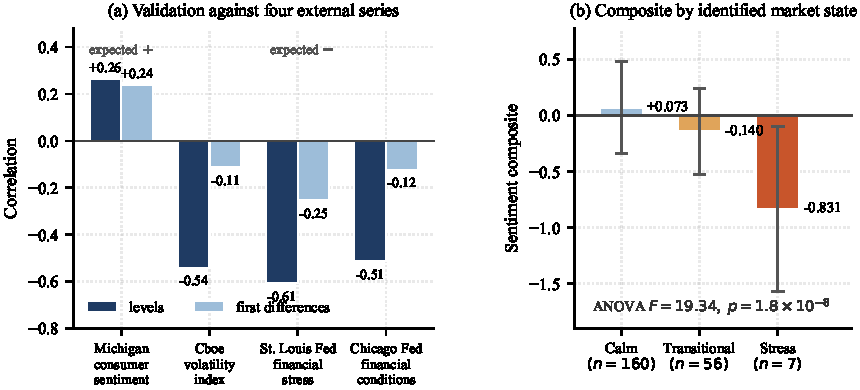
\includegraphics[width=0.95\linewidth]{figs/f_sentiment_diag.pdf}
\caption[Sentiment composite diagnostics]{Sentiment diagnostics. (a) Correlation of the
sentiment composite with four independently published series in levels and first differences.
(b) The composite evaluated by identified market state; the states are labelled by fitted
volatility and the composite plays no part in fitting them.}
\label{fig:sent}
\end{figure}

\textbf{Separation across market states.} If the identified states are states of sentiment as
well as of volatility, the composite should differ across them. Figure~\ref{fig:sent}(b) shows
a monotone and steep ordering: $+0.073$ in the calm state, $-0.140$ in the transitional state
and $-0.831$ in the stress state. One-way analysis of variance gives $F = 19.34$ with
$p = 1.8 \times 10^{-8}$, and the rank-based Kruskal--Wallis test, safer given only seven
observations in the stress state, gives $H = 29.54$ with $p = 3.9 \times 10^{-7}$. Since the
mixture model is fitted on realised volatility and short-horizon momentum, and the composite
is not among its inputs, this separation on a withheld variable justifies describing the
states as sentiment-and-volatility states rather than volatility states alone.

\textbf{Noise and lead--lag structure.} In \pubcite{P3}, the temporal overlay of sentiment
against price shows that strong sentiment spikes frequently precede major price changes, but
that the mapping from magnitude to direction is not simple: sustained positive sentiment
accompanies gradual advances, whereas sharp negative spikes accompany abrupt declines. The
sentiment distribution is approximately symmetric about neutral with moderate tails, indicating
that the extraction pipeline captures genuine variation rather than producing a biased
categorical output. In \pubcite{P5}, the predictive content of the validated composite, measured
as a cross-sectional information coefficient, is indistinguishable from zero or significantly
negative depending on the period. Keeping these two results apart is essential: a composite can
measure sentiment accurately and still fail to forecast returns.

\subsection{Summary and validation of Research Objective 3}

Transparency here derives from directed causal structure rather than from post-hoc attribution
alone, and multi-scale temporal encoding makes the horizon of each signal explicit. The
framework recovers an interpretable causal graph of density 0.850 with an identifiable hub and
demonstrates that causal influence and linear correlation can diverge, which is the
justification for causal feature selection. Sentiment noise was quantified rather than assumed:
the construct was validated against four external series with the correct sign in all sixteen
series-by-period combinations and separates market states at $p = 1.8 \times 10^{-8}$, yet
carries no reliable directional information --- a distinction reported in full because it
constrains how sentiment should be used downstream. \pubcite{P2} supplies causal discovery,
multi-granularity encoding and credibilistic allocation; \pubcite{P3} and \pubcite{P5} supply
the sentiment-noise and temporal-dynamics evidence.

%---------------------------------------------------------------------
\section{Proposed Methodology for Research Objective 4}

\textbf{RO4:} \emph{To evaluate and validate the result and practical application of the
proposed model across different stock markets, exploring transfer learning techniques for
cross-market applications and validating the model against benchmark datasets and real-world
market data.}

\subsection{Design of the decision-theoretic allocation framework}

The framework converts a fused signal into an executable portfolio in a way that keeps two
decisions separate: what to hold relative to everything else, and how much total risk to carry.
That separation is what makes each layer independently testable. In \textbf{Stage~1}, nine
causal features per asset per session are standardised cross-sectionally into a technical
composite $T_{i,t}$ and a sentiment composite $M_{i,t}$, so that a value expresses how an asset
ranks against its peers on that day rather than against its own history; this also removes the
common market factor, preventing a market-wide move from registering as a signal on every asset
at once. In \textbf{Stage~2} the market state $r_t$ is identified by a three-component Gaussian
mixture over rolling volatility and momentum, refitted at every rebalance on an expanding
window of strictly earlier sessions, with components anchored by ascending fitted volatility
into calm, transitional and stress states so that labels remain comparable across refits; the
composites are then fused with state-dependent weights and a confidence term $c_{i,t}$ that
discounts assets whose composites disagree, and the fused score is placed on a return scale by
information-ratio scaling~\cite{grinold2000}:
\begin{equation}
z_{i,t} = c_{i,t}\left(w^{T}_{r_t} T_{i,t} + w^{M}_{r_t} M_{i,t}\right),
\qquad
\alpha_{i,t} = \mathrm{IC}\cdot\sigma_{i,t}\cdot z_{i,t}.
\end{equation}
\textbf{Stage~3} splits the allocation in two. Relative composition solves a constrained
quadratic program for the fully invested risky sleeve, with covariance
shrinkage~\cite{ledoit2004}, a 25 per cent position cap and a turnover penalty annualising a
one-way cost of ten basis points,
\begin{equation}
\tilde{w}_t = \arg\max_{w}\;
\alpha_t^{\!\top} w - \lambda\, w^{\!\top}\Sigma_t w - \kappa\|w - w_{t-1}\|_1
\quad\text{s.t.}\quad w \ge 0,\; w \le 0.25,\; \mathbf{1}^{\!\top} w = 1,
\end{equation}
after which total risk is set by the regime budget $w_t^{*} = k_{r_t}\tilde{w}_t$ with
$k = \{1.00, 0.75, 0.50\}$ expressed as a fraction of the sleeve's own volatility and the
residual held in cash. Scaling is one-sided, so the framework de-risks in disturbed states but
never levers up, and any performance difference is attributable to risk reduction rather than to
leverage. \textbf{Stage~4} evaluates the result by 21-session walk-forward with 10\,bp costs, an
18-cell specification sweep, matched-exposure ablation, four stress episodes, a 665-session
holdout and a secondary market universe, with Newey--West and stationary block bootstrap
inference.

Two implementation details proved consequential and generalise beyond this framework. Mixture
component indices permute freely between refits, so labels must be anchored; omitting the
anchoring step produces no error, only a silently scrambled regime series. And the risk budget
must be expressed as a fraction of the portfolio's own volatility rather than as an absolute
target, because absolute targets calibrated for concentrated equity portfolios are never reached
by a diversified sleeve and leave the regime layer present in the specification but inert ---
here binding in one rebalance out of 224.

\subsection{Results and discussion for Research Objective 4}

Table~\ref{tab:port} consolidates the evaluation across the primary universe, the holdout, the
specification sweep and the secondary market.

\begin{table}[!htb]
\centering
\caption[Portfolio-level evaluation across universes and periods]{Portfolio-level evaluation.
Benchmarks are rebalanced daily and charged no transaction costs, which is deliberately
unfavourable to the proposed framework.}
\label{tab:port}
\tabfont
\begin{tabular}{@{}L{5.5cm}rrrrr@{}}
\toprule
\textbf{Configuration} & \textbf{CAGR} & \textbf{Vol.} & \textbf{Sharpe} &
\textbf{Max DD} & \textbf{Calmar} \\
\midrule
\multicolumn{6}{@{}l@{}}{\textit{Primary universe: ten multi-asset ETFs, Jan 2008 -- Aug
2026, 4{,}689 sessions}}\\
Proposed regime-conditional framework & 5.65\% & 6.44\% & \textbf{0.878} &
\textbf{$-$18.98\%} & 0.298 \\
Equal-weight benchmark & 8.45\% & 13.45\% & 0.628 & $-$36.08\% & 0.234 \\
Inverse-volatility benchmark & 7.46\% & 8.78\% & 0.849 & $-$24.09\% & 0.310 \\
Equal-weight at strategy volatility & 4.19\% & 6.44\% & 0.651 & $-$18.69\% & 0.224 \\
\midrule
\multicolumn{6}{@{}l@{}}{\textit{Out-of-sample holdout: 665 sessions, Jan 2024 -- Aug 2026}}\\
Proposed framework & 12.32\% & 7.63\% & \textbf{1.614} & \textbf{$-$5.48\%} & 2.246 \\
Equal-weight benchmark & 15.44\% & 11.10\% & 1.391 & $-$10.13\% & 1.524 \\
Inverse-volatility benchmark & 11.89\% & 8.51\% & 1.397 & $-$6.70\% & 1.775 \\
Equal-weight at strategy volatility & 7.28\% & 5.32\% & 1.370 & $-$7.04\% & 1.473 \\
\midrule
\multicolumn{6}{@{}l@{}}{\textit{Specification sweep: 3 seeds $\times$ 2 covariance windows
$\times$ 3 rebalance intervals}}\\
Range across all 18 cells & --- & --- & 0.813 -- 0.956 & $-$21.1\% -- $-$19.0\% & --- \\
Cells beating the benchmark on both measures & \multicolumn{5}{l}{18 of 18} \\
\midrule
\multicolumn{6}{@{}l@{}}{\textit{Secondary universe: ten mega-capitalisation equities,
2019 -- 2026 (cross-market transfer)}}\\
Proposed framework & 17.02\% & 14.87\% & 1.145 & \textbf{$-$20.45\%} & 0.832 \\
Equal-weight benchmark & 33.52\% & 24.45\% & \textbf{1.371} & $-$33.63\% & 0.997 \\
\bottomrule
\end{tabular}
\end{table}

On the primary universe the framework raises the Sharpe ratio from 0.628 to 0.878, a gain of
40 per cent, and reduces maximum drawdown from $-36.08$ to $-18.98$ per cent, a reduction of
47 per cent, while earning a lower compound return of 5.65 against 8.45 per cent per annum. It
is a risk-reduction instrument whose return sacrifice is smaller than its risk reduction, and
it is presented as such. Against the volatility-matched benchmark it retains its Sharpe
advantage but loses marginally on drawdown, which bounds the drawdown claim precisely: the
framework reduces drawdown relative to an unlevered diversified benchmark, not relative to
every portfolio held at the same volatility. The holdout block is the strongest single piece of
evidence, because every specification decision --- universe, feature set, number of regimes,
risk budget, rebalancing interval and cost assumption --- was fixed before any session in it
was examined; on those 665 sessions the framework records a higher Sharpe ratio and a smaller
drawdown than all three benchmarks, and two of those comparisons reverse the in-sample
ordering. Three qualifications are stated alongside: 665 sessions cannot settle the question on
their own, the period contains no episode comparable to 2008 or 2020, and the framework again
earns less in absolute terms.

\begin{figure}[!htb]
\centering
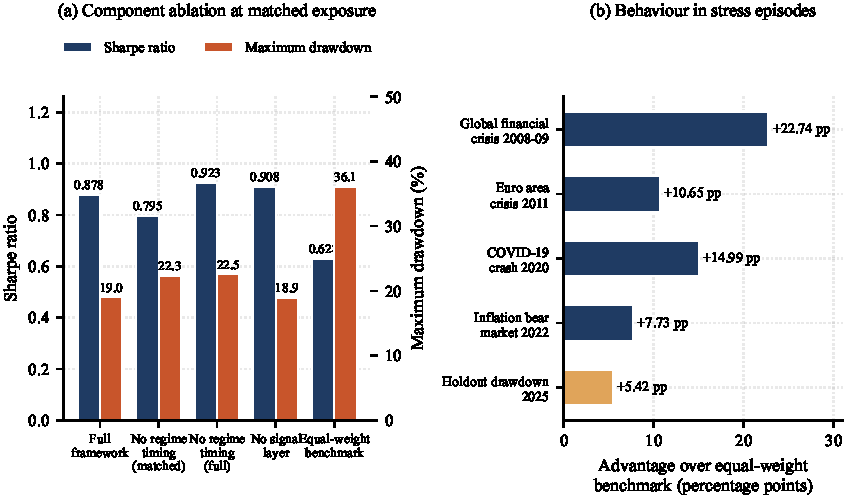
\includegraphics[width=0.95\linewidth]{figs/f_ablation.pdf}
\caption[Component ablation and stress-episode behaviour]{(a) Component ablation. The
matched-exposure control carries the same average invested exposure as the full framework but
applies it without regard to the regime, so that only the timing of risk differs.
(b) Cumulative advantage over the benchmark in four stress episodes chosen on documented
market history, plus the deepest benchmark drawdown in the holdout.}
\label{fig:abl}
\end{figure}

The ablation answers the objective's central question. Holding average exposure fixed at 92.1
per cent, allocating that exposure according to the identified regime rather than uniformly
raises the Sharpe ratio from 0.795 to 0.878 and improves maximum drawdown from $-22.26$ to
$-18.98$ per cent, with no significant difference in mean return ($p = 0.695$). That
combination --- both measures improve, mean return does not change --- is the signature of a
genuine risk-timing effect rather than of simply holding less, and it is available only because
the control was constructed at matched risk. The cost of that timing is also measured: against
a fully invested variant the framework gives up about 1.3 percentage points of annual return,
significantly so ($p = 0.016$), in exchange for 3.55 points of maximum drawdown.

The same ablation returns a null on the signal fusion layer. Removing it entirely, so that the
optimiser becomes a constrained minimum-variance problem, moves the Sharpe ratio from 0.878 to
0.908 and maximum drawdown from $-18.98$ to $-18.87$ per cent; both movements favour removal
and neither is significant ($p = 0.650$). The information coefficients explain why: the
technical, sentiment and fused composites are all significantly \emph{negatively} related to
next-session cross-sectional returns over the full sample ($\mathrm{IC} = -0.030$, $-0.026$ and
$-0.033$; Newey--West $t = -2.14$, $-2.26$, $-2.42$), and the state-dependent weighting
hypothesis --- that sentiment becomes relatively more informative under stress --- is not
supported, with point estimates running the other way and the calm-to-stress contrast
insignificant ($t = -1.46$, $p = 0.145$). The relationship is not stable enough to exploit by
inversion either: $-0.039$ before 2024 and $+0.009$ afterwards. This null is retained in full.
Component-level negative results are rarely published, which is one reason architectures
accumulate layers whose contribution has never been isolated; reporting which layer works is
more useful than an aggregate number that conceals the distinction.

Behaviour under stress is consistent across four episodes selected before the analysis on
documented market history rather than by inspection of results. The framework outperforms in
all four, by between 7.7 and 22.7 percentage points, and by a further 5.4 points in the deepest
benchmark drawdown of the holdout. Its average return on the worst 5 per cent of benchmark
sessions is $-0.59$ per cent against $-2.01$ per cent, a cushion of 1.42 points per session,
and downside capture of 0.38 against upside capture of 0.41 gives a capture ratio of 0.93: the
framework participates less in both directions in roughly equal proportion, so its advantage
comes from carrying less risk in adverse states rather than from directional skill. On
statistical significance the report is equally direct. The Sharpe difference of $+0.250$
carries a 95 per cent bootstrap interval of $[-0.102, 0.574]$, which includes zero, and the
shortfall in mean return is not significant ($p = 0.171$). Eighteen years of daily data contain
only four independent observations of the events that matter for a drawdown claim, and no
amount of daily sampling converts that into statistical power. What is robust is consistency,
not the point estimate: the Sharpe advantage appears in 18 of 18 specifications, the drawdown
advantage in 18 of 18 specifications and 18 of 19 calendar years, and the outperformance in all
four stress episodes. Robustness and significance are different properties and are not
conflated here.

\subsection{Cross-market transfer}

Transfer was tested by running the framework without modification on a second universe of ten
mega-capitalisation United States equities over 2019--2026. The outcome is mixed and is reported
as such. The framework loses on risk-adjusted return, 1.145 against 1.371, and gives up 15.09
percentage points of annual return, significantly so ($t = -2.791$, $p = 0.005$). Its defensive
behaviour nevertheless survives intact: maximum drawdown improves from $-33.63$ to $-20.45$ per
cent, it wins on drawdown in eight of eight calendar years and in all 36 specification cells
examined on that universe, and it outperforms in both stress episodes the window contains, by
12.50 percentage points in the 2020 crash and 12.60 points in the 2022 bear market. Critically,
the regime layer continues to behave as designed: against the matched-exposure control it
improves both the Sharpe ratio and the drawdown, so the risk-timing effect reproduces in a
universe where the framework loses overall.

One point of scope should be stated plainly rather than glossed. The objective refers to
\emph{transfer learning}; what has been carried out here is \emph{direct transfer}. The
framework, its feature definitions and its fitted procedure were applied to the second universe
without modification and without any adaptation step --- the stricter test of whether the
mechanism itself generalises, since no parameter was fine-tuned on the target market, no
representation was pre-trained and re-used, and no domain-adaptation objective was optimised.
The result is therefore a lower bound on cross-market performance, and adaptation-based transfer
is identified as open work in Section~7.2 rather than claimed here. The explanation is a
property of the universe rather than of the framework: ten mega-capitalisation equities are
close to a single factor bet, with high correlations, no low-volatility asset to rotate into,
and a risky sleeve carrying roughly 15 per cent annualised volatility against 6 per cent in the
multi-asset case, so de-risking can only move capital to cash and the framework systematically
forgoes return during an exceptional advance. The transferability condition is therefore
explicit and testable in advance: the framework requires a universe with genuine dispersion in
asset volatility. Complementary cross-market evidence at sectoral granularity comes from the
ten-sector evaluation of \pubcite{P1} and the sector-level regime behaviour of \pubcite{P2}.

\subsection{Summary and validation of Research Objective 4}

The framework was evaluated as a decision system rather than as a predictor. It improves
risk-adjusted return and materially reduces drawdown against an unlevered diversified benchmark,
sustains that behaviour on a holdout that postdates every design decision, and does so
consistently across every specification examined. Ablation at matched exposure locates the gain
in regime-conditional risk timing and returns a null on the signal fusion layer, and cross-market
transfer establishes a precise boundary condition for applicability. The limits of the evidence
--- an insignificant Sharpe improvement, few independent stress events, a lower absolute return
--- are stated explicitly. \pubcite{P5} supplies the framework, the eighteen-year evaluation, the
specification sweep, the ablation, the holdout and the cross-market test; \pubcite{P1} and
\pubcite{P2} supply supporting sectoral and regime-level evidence.

%---------------------------------------------------------------------
\section{Integration of the Individual Contributions}

The four contributions are not four independent studies with a shared subject; each was produced
in response to a limitation exposed by the one before it. Contribution~1 established that fusing
four sources improves prediction and that the value of each source is state-dependent, which
raised the question of how to weight a source whose reliability changes --- answered by the
uncertainty-weighted formulation. Contribution~2 isolated the language-model sentiment channel
and found it the most important single feature yet delivering only a bounded increment in raw
accuracy, which raised the question of whether the limitation lies in the measurement or in the
horizon. Contribution~3 answered by separating the two: the construct was validated externally
and found sound, while its predictive content was measured separately and found weak, so the
limitation is not one of measurement. Contribution~4 followed directly --- if the signal channel
is bounded, the framework must earn its value at the decision layer, and the ablation confirms
exactly this: risk timing by market state works, and the signal layer does not. The final system
is therefore not the one originally envisaged, and it is better supported for that reason.
